
The selection of producers among the worker pool can be achieved for each ledger cycle using a randomised approach. Since a producer generates a ledger state update for a ledger cycle based on transactions collected during the previous ledger cycle(s), such assignment to a node should be revealed at least one cycle ahead. \\

In fact, we use a method that reveals the list of nodes selected to be producers for a ledger cycle  using information available one cycle ahead. At the beginning of a ledger cycle $\mathcal{C}_n$, at time $t = t_{n,0}$, a pseudo-random number $r_{n+1}$ is drawn using the Merkel tree root of the ledger state update produced one cycle ahead ($\mathcal{C}_{n-1}$), as seed to the pseudo-random number generator. The random number $r_{n+1}$ is then used to define the list of workers selected to become producers for the next cycle $\mathcal{C}_{n+1}$ in the following way: for each worker node identifier $Id_i$ the quantity $u_i = Id_i \oplus r_{n+1}$ is defined, where $\oplus$ is an XOR function (for binary-based modulus addition). The list of new identifiers $\{u_i \}_{i=1,...,N}$ ($N$ is the total number of nodes in the worker pool) is sorted in ascending order and the first $P$ identifiers in that list are the identifiers of the nodes selected to be producers for the next cycle $\mathcal{C}_{n+1}$.\\


In a large network, it can be anticipated that a large number of nodes have available resources to be used to manage the ledger database and try to join the worker pool (which translates as a high demand for work). The size of the worker pool must however be determined by security as well as economical factors. Indeed, it must be profitable for a node to join the worker pool. Said otherwise, the average number of tokens earned by a producer over a period of time should at the very least cover its operational cost. As there might be more nodes willing to work than required for the worker pool, nodes may join a secondary pool, \textit{a.k.a} a worker queue, and wait to be called to join the worker pool. In order for these nodes to join the worker pool, there must be a mechanism that limits the time period during which a node can persist in the worker pool. The approach considered is to grant nodes joining the worker pool a worker pass which is valid for a limited period of time. \\

\begin{comment}
For security reasons explained in section~\ref{Sec:ConSec}, rather than defining a strict expiry time, a decay rate is used to determine the validity of a worker pass. Similarly to unstable nuclear elements the work pass has a 50\% chance to remain valid after the worker sits in the worker pool for a period of time equal to the its worker pass mean lifetime (see section~\ref{Sec:PassVal}). The decay rate is not fixed over time but instead can vary depending on the quality of work performed by the worker when acting as a producer. It can also vary to account for the demand for work, \textit{i.e.} the length of the worker queue, although a threshold is considered to mitigate the risk of a malicious entity (or group of entities) trying to simulate a highest demand for work than reality.\


The list of identifiers of nodes in the worker pool can be maintained in a hash table ($DHT_w$) distributed across the network. Such table also stores the decay rate of each node worker pass. At the end of a ledger cycle, nodes in the network can therefore deduce the list of worker passes which validity has expired. Nodes on the network can update the table, freeing some slots that can be occupied by the nodes sitting in the worker queue. \\
\end{comment}

The list of identifiers of nodes in the worker pool can be maintained in a hash table ($DHT_w$) distributed across the network. Such table also stores the time of issuance of the node worker pass. At the end of a ledger cycle, nodes in the network will be able to verify which passes are no longer valid and have expired. Nodes on the network can update the table, freeing some slots that can be occupied by the nodes sitting in the worker queue. \\

By providing proof of their available resource to the network \cite{coremark,pos}, nodes can freely apply to become workers: they join the worker queue. Every node on the network can store such proof alongside the node identifier in a secondary distributed hash table ($DHT_q$). As nodes leave the worker pool, nodes from the queue can join it. Assuming the list of identifiers sorted chronologically in $DHT_q$, a logic can be implemented such that nodes with identifiers at the top of the list are the first ones to access the worker pool. \\

Such an approach could be seen as potentially accommodating Sybil-identity attacks~\cite{sybil}, however expensive, if an entity controls a large number nodes at the top of the worker queue (at least equal to half the worker pool size $N/2$) and frequently adds many nodes to the worker queue such that the size of the worker queue is large enough to create an impression of a large demand for work. The peer identification protocol on Catalyst network is designed to limit the number nodes on the same IP address entering a pool of nodes. 

\begin{comment}
In particular the Ipv4 address space is small and limits the ability of an entity to spin up multiple nodes on different IP addresses. There is an exponential cost associated to get the number of distinct Ipv4 addresses needed to have enough nodes in the worker queue. \\
\end{comment}

We nevertheless consider an alternative approach to define the dynamic of nodes leaving the worker queue and joining the worker pool that both prevents Sybil attack and incentivise nodes to join the worker queue during periods of low demand for work. We propose a method to sort out the nodes listed in the worker queue. A ranking (or score) is associated to a node when it joins the worker queue. The nodes in the worker queue are then ordered based on their ranking in descending order, \textit{i.e.} the nodes with the lowest ranking are at the top of the queue and the first ones to leave the worker queue and be selected to join the worker pool when some slots are freed in the worker pool. The method to assign a ranking to a node joining the worker queue is not purely chronological-based. It depends on the volume of nodes joining the queue during same allotted time period $\Delta t$. Assume $S_t$ nodes applying to join the worker queue during a small window of time $[t, t+\Delta t]$. The $S_t$ nodes first register to a tertiary queue, $DHT_s$. At the end of the time window, a fixed and limited number of nodes from $DHT_s$, $z \leq S_t$, are randomly selected. $z$ is equal to the number of nodes who left the worker pool during the time window  $[t-\Delta t, t]$. These $z$ nodes are given a ranking drawn from a normal distribution centred around $R_q$, which is a predetermined threshold of the worker queue length. This means that some selected nodes may obtain a ranking higher than nodes currently at the bottom of the worker queue. The rest of the nodes in the tertiary queue ($S_t-z$) are given a ranking drawn from a normal distribution centred around $R_l = R_q - s$, where $s$ is a shift inversely proportional to the volume of nodes in the tertiary queue $DHT_s$. Figure~\ref{fig:NSM} illustrates the process of ranking allocation for nodes joining the worker queue. \\
%The rotation rate of nodes in the worker pool then depends on the size of the worker queue but only take into account the number of nodes with a ranking higher than a given threshold. 

\newpage
\begin{landscape}
\begin{figure}
\centering
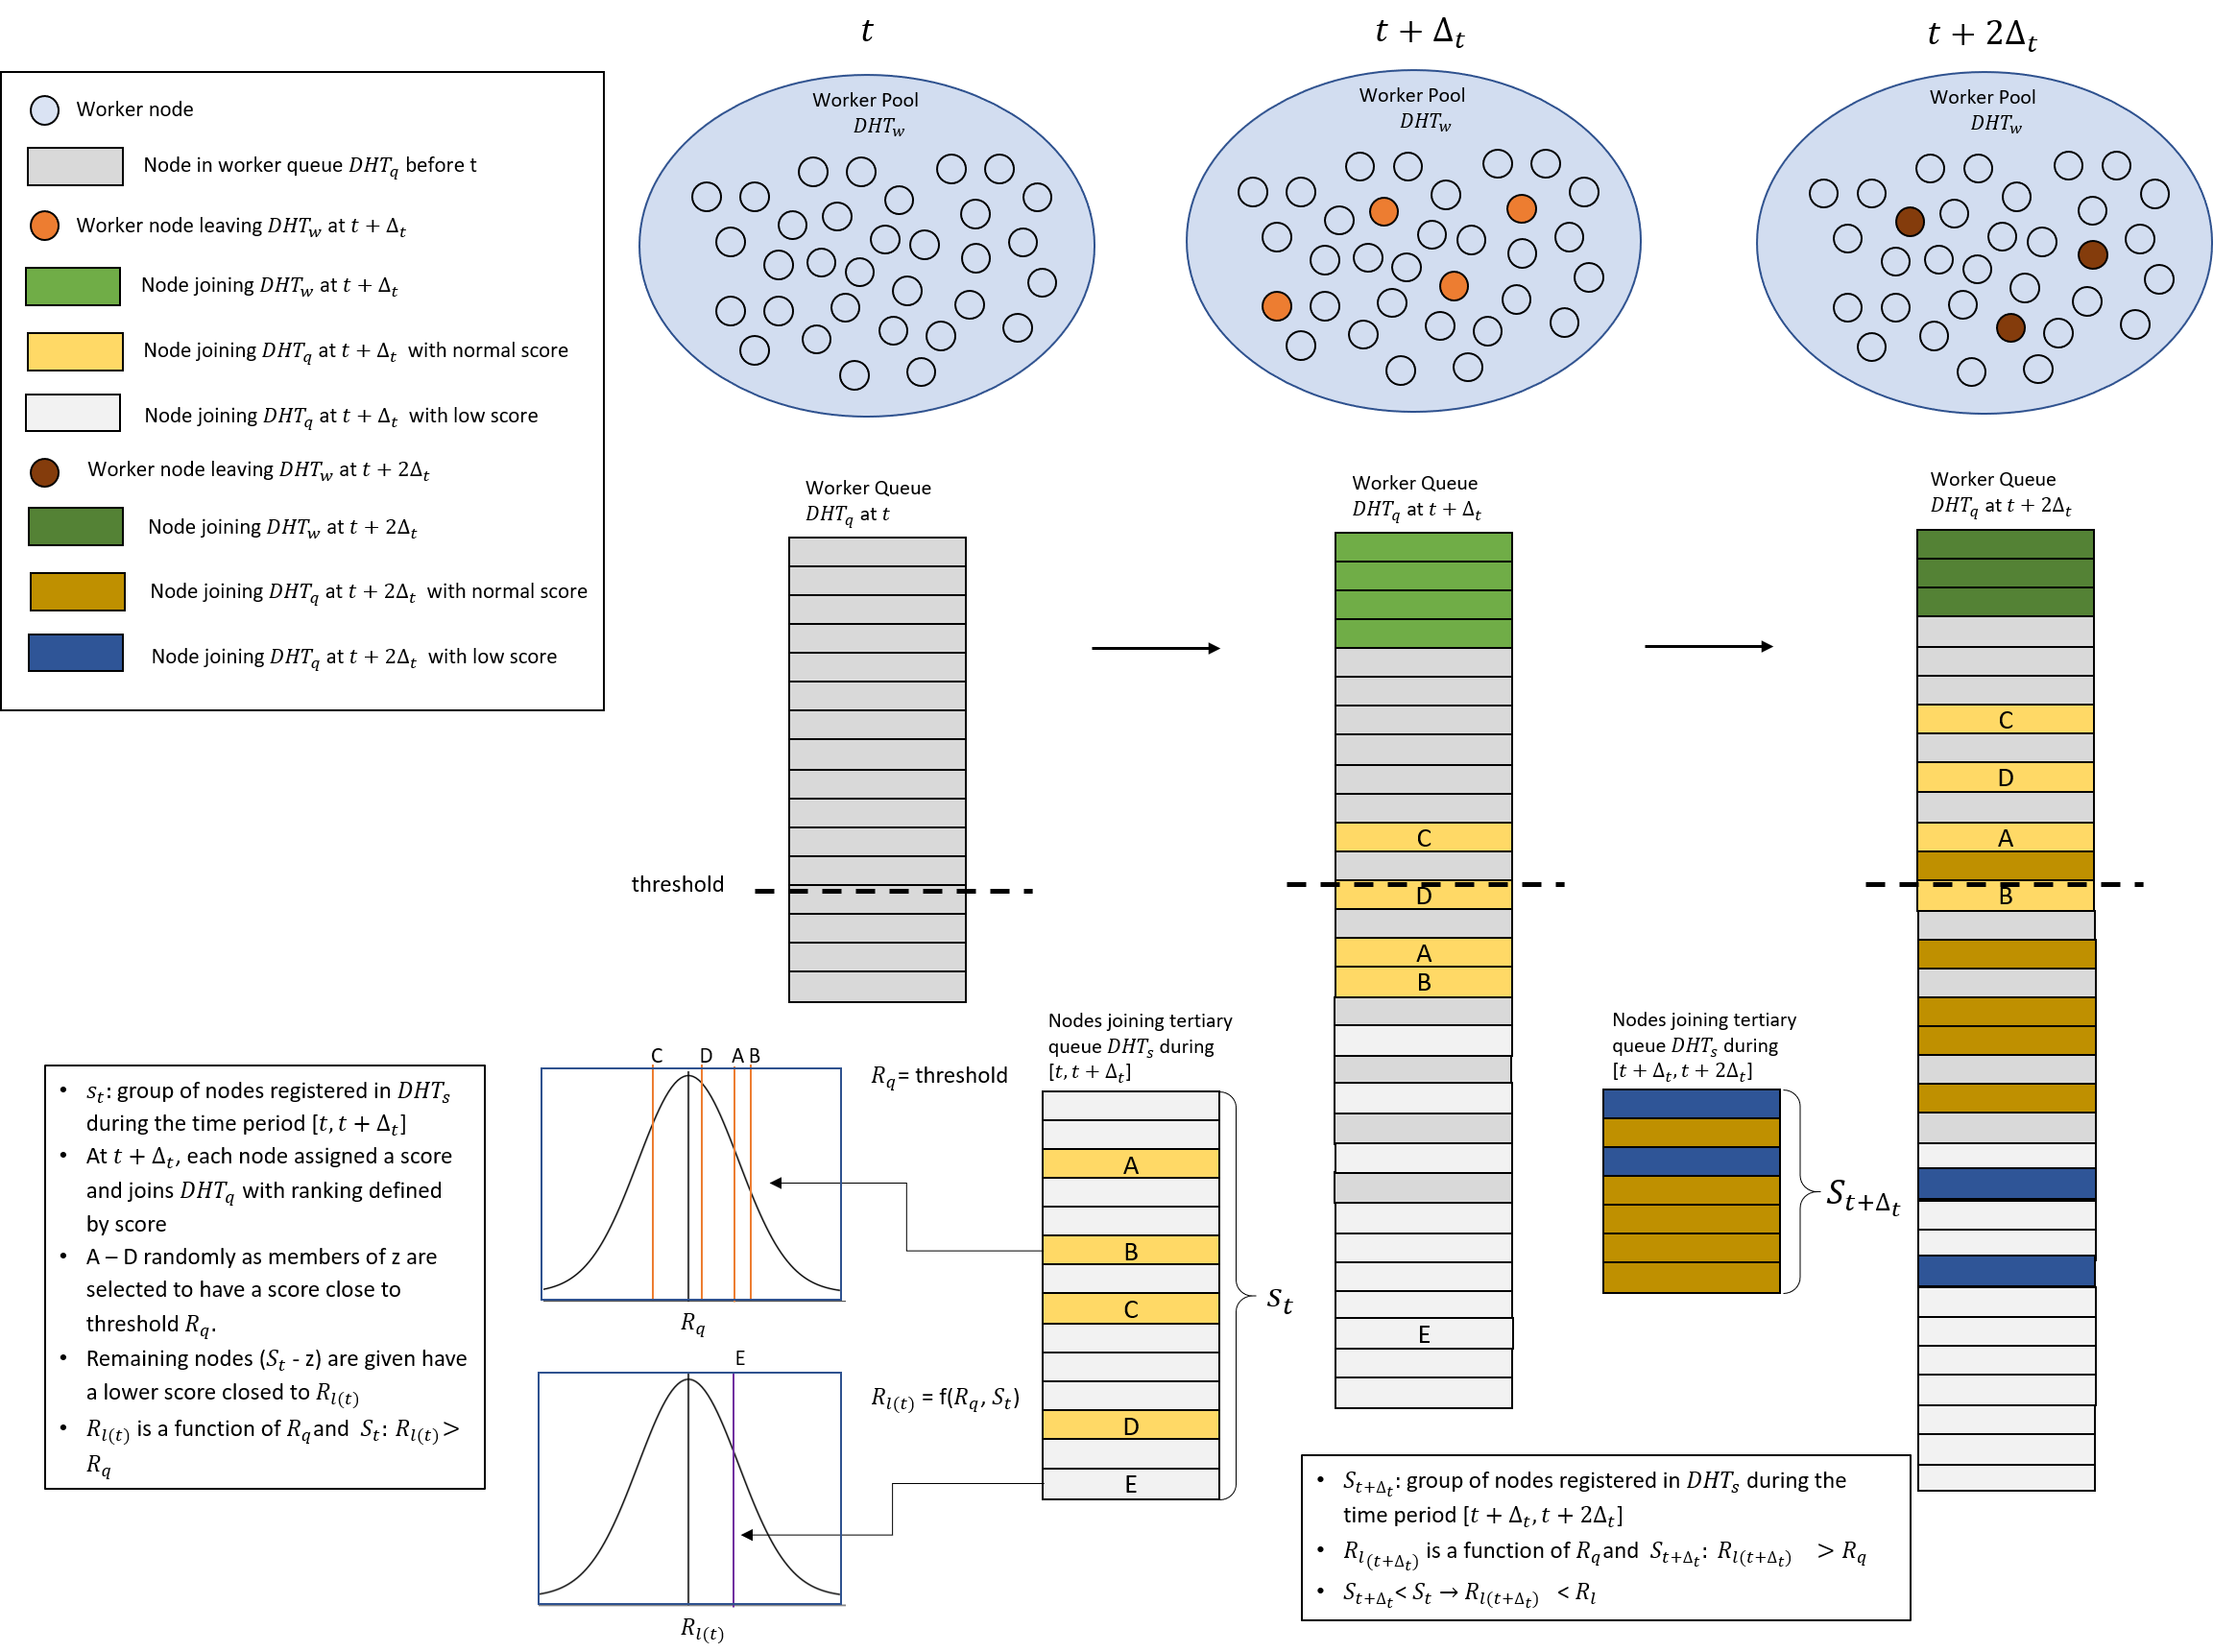
\includegraphics[width=22cm,height=42cm,keepaspectratio]{Figures/Work_Queue_Management}
\caption{\label{fig:NSM}Illustration of the process followed by Catalyst network to add nodes to the worker queue.}
\end{figure}
\end{landscape}

